% \newcommand{\jarule}{\vskip 1em \centering \hrule height .2pt depth .2pt width 2in \vskip 1em \par}
\newcommand{\jarule}{{\centering \vskip 1em \rule{0.5\textwidth}{0.5pt} \vskip 1em \par}}

\newcommand{\sectioncount}[1]{\vskip 1em \textbf{#1}.}

\chapter{The Repressed Content-Requirements of Mathematics (1987, 1994)}

\textbf{A.} Mathematics, as it is conceived in the twentieth century, has presuppositions about perception, and about the comprehension of lived experience relative to the apprehension of apparitions, which are repressed in professional doctrine. It also has presuppositions of a supra-terrestrial import which are repressed. The latter concern abstractions whose reality-character is an incoherent composite of features of sensuous-concrete phenomena.

In the twentieth century, mathematicians have been taught to say by rote, \enquote{We are beyond all that now. We are beyond psychology, and we are beyond independently subsisting abstractions.} This recitation is a case of denial. Indeed, if this recitation were true, it would allow mathematics nowhere to live. Certainly social conventions---beloved by the Vienna Circle---are too unreliable to found the truths which mathematicians claim to possess. (Truths about the decimal value of $\pi$, or about different sizes of infinity, for example.)

To uncover the repressed presuppositions, a combination of approaches is required. (One anthropologist has written about \enquote{the locus of mathematical reality}---but, being an academic, he merely reproduces a stock answer outside his field, namely that the shape of mathematics is dictated by the physiology of the brain.)

The competence called \term{counting} is required in mathematics. But such counting is paradoxical \enquote{phenomenologically.} The first portion of my conclusions concerns the phenomenology of counting, with particular reference to enumeration in the life-world.

Mathematics as an activity of thought has a \enquote{phenomenology.} I'm not even referring to the \enquote{discovery} of new knowledge. Just the successive contemplation of terms of a series, or the counting of abstract entities, as may happen when reviewing a proof, has a paradoxical phenomenology. Brouwer made explicit and incredible claims for mathematics as a mental activity.

Realistically, also, the comprehension of an important proof is quite unlike the mechanical checking of a formal proof. So a portion of my conclusions concerns the phenomenology of abstract ratiocination.

Husserl attempted to \emph{defend} mathematics on a psychological or phenomenological basis. But that is not at all what I do here. I'm not an apologist for mathematics. I have no motive to protect its claim to be knowledge. Indeed, I argue that the abstract rigidity of the mathematical elements, combined with the mystical obscurity of infinite structures, is a delusion associated with a specific lineage of civilizations. I am investigating this delusion not because I want to protect it, but because I want to exit to a different civilization.

To continue, mathematicians' intentions require a realm of abstract beings. (Frege, G\"{o}del, Quine, etc., admit the need to assume the non-spatial, abstract existence of classes.) But mathematicians are unable to expound the tenet of celestial existence of abstractions. Not since the seventeenth century, perhaps, has anyone attempted to provide a supporting metaphysics for whole numbers, geometric figures, and infinities. In this connection, a portion of my conclusions concerns the repressed content-requirements regarding independently subsisting abstractions: whole numbers, geometric figures, etc.

No twentieth-century philosopher of mathematics has dared to undertake the substantiation of e.g. whole numbers as celestial beings. (Whole numbers are explained as formal terms or numerals in a network of rules.) \emph{And yet}, naive arithmetic continues to be used---along with the language of words in which theories are expounded.

At the beginning of the twentieth century, Hilbert convinced the profession to conceive consistency as the paramount question of the validity of mathematics. Another portion of my observations will concern how the content of mathematics is molded by the choice of allowable proof-methods, and by tendentious adjustments to the definition or test of consistency.

\jarule

\textbf{B.} It is a lesson in intellectual history that mathematicians have been taught to say by rote, as I noted above, that \enquote{we are beyond all that now.} The enterprise of foundations of mathematics was contrived to push Platonic questions and psychological questions underneath the \enquote{trading floor} of frenzied effort---where it was hoped that they would remain unnoticed. In other words, foundations of mathematics, which promised to find the bottom of mathematics, pushed the real bottom under the floor and hoped that it would remain unseen.

Also, foundations of mathematics evolved as an intricate computational science \emph{inside of} number theory. The mirage was cultivated that intricate computational exercises in different degrees of infinity, and so forth, could validate our right to do naive elementary arithmetic as it is done in the present civilization.

A minority among the foundationalists additionally learned to say by rote: we are beyond Platonism, we are beyond extensional logic, we are beyond impredicativity, we are beyond nonconstructibility. Again---as long as we are talking about published research with a professional career\footnote{Errett Bishop, Nicolas Goodman, Edward Nelson, Michael Beeson, etc.}---the claims to be \enquote{beyond it all} are instances of denial. Again, mathematical truth is demanded to have a rigidity, an absoluteness, that is tantamount to Platonism. Again, the Platonic, logic-of-actuality base of the supposed novelties is pushed under the floor, where it is supposed to live unseen.

A notable lesson is provided by D. van Dantzig's paper on what is essentially Brouwer's inconsistency proof of classical analysis.\footnote{\papertitle{Comments on Brouwer's Theorem on Essentially-negative Predicates,} \journaltitle{Indigationes Mathematicae}, Vol. 11, pp. 347--55.} In the first place, van Dantzig does not say that the topic is an inconsistency proof; evidently that would be too provocative. In any case, the paper is almost the only one ever published which sketches the heretical agenda which Brouwer's subjectivism would introduce. I have appended the key pages from the paper to my Bibliography. Is the mathematician's death a result in mathematics? What if two mathematicians disagree about what is a proof? van Dantzig lists these issues under the heading \enquote{Terminological remarks.} They are only terminology, he tells his readers, and so they are quickly thrust aside. The pretense of eternal, super-human truth persists because it is professional suicide to drop it.

Even those who claim that mathematics is a purely syntactical discipline are unable to avoid content---or to avoid naive arithmetic
\begin{itemize}
\item in syntactical enumeration;
\item when positing that a symbol can be an abstraction;,
\item when demanding that rules must address classes of cases.
\end{itemize}

\jarule

\textbf{C.} Let me focus on Hilbert's program. For Hilbert, the whole of mathematics came down to the consistency of uninterpreted calculi. Let me spell out Hilbert's problematic to see where it stands relative to the repressed content-requirements.

One posits an \term{a priori} conceptual system embodied in language and symbols.

Is the system defined by contents (i.e. a pre-established realm of abstract referents)? Or---is the system defined by rules? \textit{[syntactical infinity]}\footnote{See the inset remark below.}[As in the stock analogy with chess---which is discussed by Frege if not prior to him.]

The system is codified in token-strings whose purpose is to assert. (Strings called propositions.)

The derivation of certain classes of propositions from other classes of propositions is mandated (by the system or in the system). But then the abstract objects called classes are required to exist. \textit{[syntactical infinity]}\editornote{sic}

The system has classical negation. The preferred intuitive picture of negation is that it is the splitting of a universe of discourse in two. But this is a definition by model, which has to be translated into status-of-propositions. In the sectarian jargon, when a universe of discourse is exhausted by set $A$ and its complement $~A$, then `$x\in A$' is true if and only if '$x\in\lnot A$' is false. [The interrelation of set complementation, negation, and truth.]

The system has an infinity of objects or terms. \term{[syntactical infinity]}\footnote{Whatever that may mean. The notion of splitting a universe of discourse into exhaustive disjoint sets becomes weirdly problematic when infinities are admitted. Now there are particular objects you will never see.}

[An entire separate branch. I presented a prima facie objection to infinity of terms, and to classical nonnegative integers. \essaytitle{Intuitive Objections to Numerical Infinity} (1991).]

The outcome, in Hilbert's doctrine: the fate of all of mathematics hangs on a single question. \textbf{Can the a priori conceptual \textit{system} be refined until it becomes \textit{impossible} for a proposition and its negation both to be derived?} Impossibility of $\vdash A$ and $\vdash\lnot A$?

What happens in this approach is that the consistency judgments become the locus of the negotiation. Manipulations of judgments of consistency become the source of mathematical content. I will return to this phase at the end.

\textbf{\textit{Syntactical infinity.}} How can one speak of having an infinity of terms if `[infinity]' is not given except as an uninterpreted sign within the game?

Foundations of mathematics takes as its problem to start from nothing and vindicate the concept of infinity. In order to do this, it assumes infinities in the world---without being able to say what that means---so that these infinities can provide a lexicon or semantics for the formal axiom of infinity. Bolzano, Dedekind, Tarski. Tarski sweeps these questions into footnotes. They are \enquote{difficult questions,} but also \enquote{superfluous complications.}\footnote{\booktitle{Logic, Semantics, Metamathematics}, pp. 174, 282.}

How can one speak of a symbol as an abstraction---unless there is a realm of abstract objects which are \textit{mathematical} objects, or are just like them?\footnote{Carnap says in \booktitle{Logical Syntax of Language} that the letter \enquote{o} is the geometric figure called a circle---the Platonic figure. Tarski dances around the question in \textit{op. cit.}, pp. 156, 174, 282.}

Rules have to address classes of cases: classes have to exist.

\jarule

\textbf{D.} My commentary is addressed in the first instance to a tradition which devolves from Platonism by the formalist route. As for L.E.J. Brouwer, he claimed that he conceived mathematics as a languageless, solipsistic activity of consciousness. It is an elementary exercise to show that Brouwer's subjectivism was either untenable or insincere. After all, Brouwer claimed the absoluteness of mathematical truth as vehemently as anyone else.\footnote{I have a manuscript, \essaytitle{Brouwer's Inconsistency Proofs of Classical Mathematics} (August 1988).\editornote{Henry Flynt has this, but we don't.}}

But all that is a distraction in this inquiry. Brouwer and his adherents claim that he is the one man in three thousand years who has nothing in common with the others---and who gets it perfectly right every time. It is all too familiar: for academics to claim to overturn the world via an application of prejudicial skepticism.\footnote{I have a manuscript on prejudicial skepticism.\editornote{We're jealous.}} We shame ourselves when we humor the professors' self-importance. This manuscript addresses the entire enterprise of mathematics; it seizes the crisis in foundations of 1900 as an object-lesson, but is in no way confined to that crisis.

{ \itshape Note on sources. I propose in this manuscript to discuss questions which are rationally defined and do not have to be referred to specific authors. Mathematical knowledge is not supposed to depend on the word of a particular authority---on citations which have the character of Biblical verses. I will keep citations to a minimum. The references which substantiate my claims about how issues are construed by the profession are collected at the end. The reader is welcome to read all references cover to cover.}

\jarule

\section*{E. Phenomenology of Counting}

Let the question be the one asked in foundations of mathematics: do we have the right to do elementary arithmetic as we do? Let us cancel the right of pure mathematicians (and foundations-of-mathematics specialists) to rig the \enquote{disputation} on this question. Let us begin an inquiry on this question which is not pledged to protect any one disciplinary orthodoxy.

When it is said that the same numbers count
\begin{itemize}
\item emotions
\item shadows
\item wooden blocks
\item hours elapsed
\end{itemize}
is that supposed to be a absolute law self-evident to consciousness from the beginning of time? There is no such thing as a proof, prior to all thinking, that the positive integers exist as abstractions capable of attaching themselves to every apparitional situation which involves plurality.

Greek philosophy claimed notions to be self-evident which not only are not self-evident, but are not evident at all, to most cultures. (Frege claimed precisely that whole numbers are universally applicable. His treatment already pushed the life-world competance of reckoning under the floor.)

\jarule

What does it mean when, in the process of \enquote{comprehending} lived experience, one counts \enquote{apparitions}?

When two shadows suddenly become one, did two shadows coalesce and persist in superposition, or did one shadow stop existing while the other survived? If we choose sense-specific apparitions as our \enquote{entities} (or \enquote{isolates}), then these isolates do not behave as things: they are evanescent. I can discard \enquote{positions,} or images, in my visual field by turning my head. So the images are evanescent (somewhat like soap bubbles). Arithmetic is not an abstract representation of the way \textit{phenomena} cumulate. Arithmetic is a sort of imaginative violence which remakes the phenomena into fixed unit-things. Teaching arithmetic is a matter of instilling, as natural, the habit of identifying\\
\parbox{4.25in}{\vskip 0.75em \centering\itshape combination of abstract units \vskip 0.75em}\\
and \\
\parbox{4.25in}{\vskip 0.75em \centering\itshape combination of concrete phenomena \vskip 0.75em}\\
---when they are manifestly divergent. So applied enumeration resembles the delusions induced in experiments in hypnosis.

Explicit counting must be carried out temporally, using tokens which appear and disappear in time. I count a manifestation of simultaneously present, persistent \enquote{things} by pairing them with a succession of thought-events which appear and disappear in time. By the time I think the enumerative token \textit{two}, \textit{one} is gone. What is supposed to make the result of this procedure meaningful? The empirical possibility of mathematics depends not as much on stable notation-tokens as on evanescent notation-tokens, since explicit counting is carried on with evanescent tokens.

In order to sustain belief that $1+1=2$ is validated by the way concrete things taken as units cumulate, you have to select the aspect in each case that agrees with $1+1=2$.

If you count simultaneously present, enduring entities by a purely mental procedure, then the entities are viewed under the aspect of endurance, while the procedure of numbering them takes place under the aspect of flux (since the silent counting labels \textit{one}, \textit{two}, etc. successively happen and vanish). So different \enquote{sides} of \enquote{the world} are apprehended under mutually exclusive world-aspects.

When you count a (displayed) unsymmetrical stable multitude by an exclusively mental procedure, you assign to the members a succession of thought-events which appear and disappear in time (exhaustively and without repetitions, which means that the procedure is also an ordering). One apprehends different \enquote{sides} of \enquote{the world} under mutually exclusive temporal world-aspects.

If you count via the expressions in a memorized sequence whose number-assignments you don't know immediately, then the procedure will yield an expression, but will not of itself tell you the number. Using the English alphabet, what is it that makes $s$ intend differently from the label $19$?

For quantity to be felt to be a reliable property, one must be surrounded by phenomena conceived as enduring and changeless (and discrete). But one's sensuous experience of a stone is fluid---and intermittent---so that at the least, an interpretation is required to extract the enduring, changeless stone from the impressions. Moreover, the counting labels have to comprise a fixed protocol, accessible by repetition. Yet \enquote{the world} has to be a flux for enumeration to be a process of comprehension. Various countings actively substitute, for the given problem, a different problem which has the character of inertness and discreteness. The establishment of equinumerousness between phenomena having different reality-statuses is crucial in supporting quantity as a property. The required permanent, discrete objects, and their required relationship to the flux-aspect and to repetition, have to be willfully imputed. Mathematicians would not be able to imagine their ideal numbers if they could not interpret their surroundings as allowing permanence, flux, and their interconvertibility, as I have discussed.

\jarule

One can apprehend temporality under the aspect of world-endurance, and also of world-flux (as events, and world, appear and then disappear into the past). Endurance and flux are both \emt{totalized} world-conditions. There was a philosophy---its name doesn't matter now---which said that we always deploy both vantage-points at once. What is more, it was said, there is no problem of logical conflict between the vantage-points. So what is claimed? On the one hand, an enduring world in which positional relationship---configuration---is supreme. On the other hand, a world which vanishes into the past and appears anew at every moment, in which sequence is supreme. The now-forgotten philosophy evidently said that the uniting of these mutually exclusive world-aspects is the precondition for there to be any cognitive apprehension whatever. The lesson is that when one excavates the constituents of elementary thought in order to validate them, one sinks deeper and deeper into quicksand.

\jarule

One may record the lapse of a multiplicity of full moons by marking a permanent surface (a rock face) at each full moon. In this case, the transitory events are so much separated that they can only be compared in recollection; moreover, memory is not a convincing medium to cumulate the observations of dozens of full moons. So a \enquote{repeating event} with a period far outside the scope of an experienceable time-lapse is modelled by a display of continually and simultaneously present marks.

\jarule

Mathematics wishes to define positive whole numbers which are so ideal that they do not reflect phenomenal considerations or reality-features. It may be noted that Brouwer invoked a reality-feature: he based number on flux---the comprehension that time has \enquote{crept.} But this step is insincere, since Brouwer does not adopt any of its ramifications, such as the point that in an entirely time-directed world, nothing would be repeatable.

Even though mathematics now claims to address ideal numbers which can therefore have any assigned content or no content, mathematics is completely dependent on \enquote{real-world} enumeration at the level of counting notations (or reading stoke-numerals, for that matter). This circumstance guarantees the general observation that mathematicians would not be able to imagine their ideal numbers if they could not interpret their surroundings as allowing permanence, flux, and their interconvertibility.

The claim of the objective realism of modern arithmetic (including all the infinitary properties of the natural number series, which outrun all phenomenal considerations, and whose explicit treatment forms much of the content of pure mathematics) is a fantasy.

Insofar as mathematics uses real-world enumeration while relentlessly denying it, mathematics has produced a series of abstract explanations of number which amount to circular solutions of spurious problems. Let us leave aside the claims that the whole numbers outrun any concrete notation, and in fact comprise an infinite series. (Such claims outrun phenomenal analysis.\footnote{Except for the "psychological proof of infinity" given by Bolzano and Dedekind. The observations I make here make the rebuttal of that proof trivial.}) After ruling out what are pejoratively called psychological explanations, mathematics comes to identify the numbers with any ordered series of labels that has a first member and an infinite tail ($a'$ after $z$, etc.). It dismisses as unnecessary the requirement that the whole numbers be \enquote{equally spaced} (the intuitive metric); and it purports to determine the whole numbers without defined addition. If this doctrine were sound, then $s$ would be the same as $19$ to immediate comprehension. What we learn is that the most \enquote{basic} branch of modern pure mathematics is a nonsensical fantasy that has grown out of the repression of the phenomenal character of enumeration.

\jarule

Hans Freudenthal's \booktitle{Lincos}, one of the first studies in the field of Communication with Extra-Terrestrial Intelligence, wants us to initiate contact with advanced extraterrestrial beings by broadcasting number theory to them. What arrogance, to suppose that this is how humans should proclaim their genius to the cosmos. I am not worried that advanced intelligent beings might fail to understand the transmission because of their \enquote{stupidity} or culture-boundedness. Freudenthal's dangerous assumption is that advanced intelligent beings will admire earthlings for sending this transmission.

\jarule

\section{Abstract Thought-Processes}

Progressive specification is required to isolate ideal geometric figures from background space. Progressive specification is required for proof-constructions, including geometric superposition. Nevertheless, it is forbidden to include these mental acts as constituents of mathematics.

When sequential procedures are used, this does not mean that the mathematical objects flow and change. Rather, the mathematician's attention moves from one rigid, eternal object to the next. This movement of attention is excluded as a constituent of mathematics.

Mathematics requires mental acts, conceptual steps, to be carried out uniformly and without resistance an infinite number of times.

\jarule 

\section{Concrete Imprints of Thinking}

The signs, notation-tokens of mathematics, are forbidden to yield different images to different people, or yield different images at different times.

Inasmuch as geometry depends on representing positional relationship in a extended field by the practice of drawing, there must be an equivocation between ideal entities, and the proxies for them which are produced by drawing. By definition, a tangent to a circle actually intersects the circle; it is not merely adjacent to it. Protagoras held that knowledge can only concern the perceptible. He observed that a palpable tangent to a circle in fact touches the circle not at a single point, but always along an arc.

Drawing requires actual motion and involves figures which evolve in time.

An intention is required to make a flat drawing into a figure of plane geometry, as opposed to a figure of solid geometry (also to understand that the figure remains flat when a page is bent, etc.). It is forbidden to include intentions as constituents of mathematics.

\jarule

\section{The Reality-Character of Pure Whole Numbers and Euclidian Figures}

Let me continue with my conclusions regarding mathematical entities conceived as self-subsistent.

% 1. Mathematical objects must be strictly separate from the self, and strictly impersonal.
\sectioncount{1} Mathematical objects must be strictly separate from the self, and strictly impersonal.

Mathematical entities have no personal specialness. Things which are partially capable of being ranked can be exhaustively linearly ranked.

Mathematical objects which are specified alike (specified similarly), are absolutely identical, without miniscule differentiations. (Ones, in a sum of ones; circles with the same radius.)

Cumulation cannot produce qualitative change.

Objects are intangible, immaterial.

Objects are rigidly self-identical for eternity.

There is no difference between possibility and actuality.\footnote{In mathematical logic, you can define an entity which is not actual; any such definition, however, is claimed to be inconsistent!} (But what about infinity?)

\sectioncount{2} Whole numbers are unextended.

Whole numbers are qualitatively homogeneous or qualityless.

Units (ones) have exactly the same magnitude.

Units retain their distinctness in combination. ($1+1=2$, not $1+1=1$.)

The series of whole numbers continues uniformly and regularly \enquote{to infinity} without confusion of identity between numbers.

\sectioncount{3} Space is that which is left when all material bodies are removed from the world.

Portions of this space can be isolated, by stipulation, from the background space, and given an identity as \enquote{figures.}

The identity of a figure persists when the figure is moved. In the first instance, only figures in a single plane are considered.

The test of equality is rigid superposition; so that figures must be movable, while retaining their identity.

Figures are absolutely intangible, may be infinitely thin, and must be absolutely permeable; but are absolutely rigid.

Superposition in plane geometry may necessitate flipping a figure out of the plane.

\sectioncount{4} Zero, the whole number for nothing. Elementary counting applies only to discrete phenomena and is done in \enquote{cells} of one---even absences are counted as positive whole numbers. \enquote{Zero} would have to mean \enquote{none} or \enquote{nothing to count.} But the situation \enquote{nothing to count} becomes a quantity which enters into computations such as $2\times 0=0$ or $0\div 0$ or $0^0$. \enquote{Nothing to count} is given the reality-character of a whole number, as declared in {\S}2.

von Neumann's interpretation of zero as Zermelo's empty set. Here a nothing---a collection with zero members---is posited to exist as a bordered (or delimited), fixed, pre-established entity. Every ontological category becomes a determinate and calculable thing, including that which by definition is not. Nothing is asserted to exist as a determinate thing. So twentieth-century scientism arrives at the very idea which Carnap railed against in his paper against Heidegger.\footnote{Note Husserl's 1891 attack on the empty set.}

Explaining \enquote{zero} as a number for nothing is not the only explanation possible. But the alternative is highly unworkable. To sketch this alternative, we have to hypothecate that counting refers to a fixed collection of tokens, say 100 tokens. Then no number above 100 can be counted. Counting becomes binary sorting of the collection of tokens: to count 3 items means \enquote{3 tokens used, 97 unused.} Now zero can be defined without any reference to nothing, as \enquote{100 tokens unused.} The total number of tokens must be fixed, because if zero were defined as \enquote{all tokens unused,} it would only create a new mystery around the indefinite word \enquote{all.} What is the cardinality of \enquote{all}? A further subtlety is that this approach works only in a universe in which possibility and actuality are the same thing. (\enquote{Zero unicorns are present} is translated to some definite positive number of unicorns claimed to be absent!)

\jarule

\section{How Allowed Proof-Methods Shape the Content of Mathematics}

I have surveyed the content-requirements of mathematics with special reference to covertly demanded metaphysical properties of mathematical entities. However, I do not suppose that these contents are really pre-established in Heaven. On the contrary, I propose that the contents arise conjointly with \textit{the method of ratiocination}. One can survey this co-conditioning synchronically, relative to a contemporary rational reconstruction of mathematics. Or, one can take history as a parable, and consider how mathematical objects were progressively focused in ancient Greece---in the wake of Thales' demand for a break with pragmatic reckoning.

Mathematics is an application of Parmenides' logicism to problems of quantity and magnitude. To establish an assertion logically has the effect of constraining vernacular concepts to rigid, literal meanings. This leads to the abstraction of a perfect line (etc.). Then Plato's question, \enquote{Where does a perfect line live? Where does an abstraction live?}

Ancient Greek thought furnishes an example that construing language dogmatically leads to conclusions which are unnecessarily paradoxical. If \enquote{one} means \enquote{wholeness,} how can there be two ones?---how can there be three ones?---etc.

Protagoras held that knowledge can only concern the perceptible. On that basis, he rejected the logicists' law of contradiction. Arrange three tanks of water in order: cold, lukewarm, hot. Put your hands in the cold and hot tanks. Then put both hands in the lukewarm tank. You feel the same water to be cold and hot at the same time. To Protagoras, that rebutted the law of contradiction.

A \enquote{cultural style} view of the discovery of mathematical theorems and mathematical proofs. Begin with a \enquote{quicksand culture} in which prohibition of \enquote{wrong} thoughts is by superstition, not by rationality.

Axiomatic mathematics: try to shrink the cultural quicksand to give unique results by rational restrictions. Some of these results are intuitively welcome; some are deeply counter-intuitive. Rig the geometry game so that the perpendicular to a line at a given point is unique. Two right angles (added) give identically a straight line.

Draw a right angle whose legs are equal segments, and draw the two circles which have those segments as diameters. The circles intersect in \enquote{right angles.} But the supplementary right angles fail to be equal anywhere but at the points of intersection---what sort of right angles are these?

If the right angles are defined by tangents, let us remember Protagoras' observation: a tangent to a circle in fact touches the circle not at a single point, but always along an arc. The Greeks already knew these and many other counter-examples to Euclidian geometry; but chose not to insist on them.

We should not read old mathematics from the standpoint of a modern mathematician who knows all the \enquote{right} answers. We should ask what it meant to them, in a non-condemnatory way.

The purpose of a proof is to exemplify and intimate all the restrictions on vernacular thinking required to produce unique results which are simple and elegant. The number of prime numbers is infinite. Every natural number is either prime or composite.

Euclidian uniqueness of the right angle is a \textit{cultural style} which is buttressed by all the explicit and implicit provisos. If the Greeks had allowed non-zero angles too small to see, their proofs of uniqueness would not work. [Also: erecting a perpendicular at a straight line's \enquote{endpoint at infinity.}]

Proof by contradiction. The objection is that you have not considered that the opposite hypothesis may also produce a contradiction. Aquinas' proof of God: infinite regress of causes is a contradiction. Why isn't a finite regress of causes a contradiction also?

Brouwer, \textit{1933}, p. 444 says that every proof of the Fundamental Theorem of Algebra was by contradiction.\editornote{I believe Flynt is referring to \essaytitle{Willen, weten, spreken $\lBrack$Volition, knowledge, language$\rBrack$}.}

Theorem and proof in Platonic mathematics. The enterprise is not reducible to legality in a game. (Formal satisfaction of the terms \emt{axiom}, \emt{proposition}, \emt{proof}, \emt{theorem}.) Parmenides' glossomorphism\footnote{Felix Cleve} is used to negotiate a world of absolute beings out of the empirical and the vernacular, the casual or flexible. The intuitively preferred abstractions, and the logic of proof, are co-determined.

The uniqueness of the perpendicular to a line at a given point is proved by contradiction. Simultaneously adjust the determination of the geometrical figure, and the logic of proof, to give the preferred result.

Formal proof is like the positivist explanation of scientific theory as an interpreted formal calculus. It's not enough. The formal calculi which mathematicians take seriously have traditional mathematical content smuggled in somewhere---it's invoked in the meta-language, for example. (Finsler and Brouwer protested that a formal proof is not a genuine mathematical proof.)

Proof of infinity of primes in Euclid etc. The mathematician thinks he discovers constructive or computational tricks which enable him to directly see intricate regularities in infinite collections of abstractions. In fact it is only a guess, or a program for what rationalism wishes to be the case.

Such a seeing of regularity in the infinity of abstract objects is an illusion. There is also a strong component of \enquote{God won't deceive me} in the method. God won't make a truth which seems to have a clear proof, but later fails because of a tiny loophole. Well, what about the loopholes in Euclid's geometry that M. Pasch closed two thousand years later, the axioms of order? Glaring loopholes that Euclid overlooked, for some reason. The mind-boggling denouement of Frege's \booktitle{Grundgesetze}. He writes for pages about how lucid, transparent, exact, and precise his work is; then confesses in an Appendix to Vol. ii, added as the work was going to press, that his system has been wrecked by Russell's paradox.

The \enquote{rationalist} (Plato, Descartes) believes in an objective abstract realm which he can know because the ostensible truth is not misleading. Consider the tenet of chess that a king and two bishops cannot mate against a king. The tenet can be disproved if a computer is used, and large numbers of moves with no humanly discernable theme or purpose are allowed. The formal approach with a powerful computational machine (to a finite problem in abstract pattern) rebuts the result obtained by rationalism.

A proof may be pictured as making a guess plausible. (The number of primes is infinite.) In classical logic, that gives $A$ credibility over $\lnot A$. But also: The allowed method of proof creates content in the Heaven of numbers. The content of the Heaven of numbers is not unaffected by what proof-methods are allowed.

Does the effort to obtain unique answers produce \textit{new contradictions}? It definitely produces new \enquote{failure theorems.}\footnote{The coinage I expound in \essaytitle{Anti-Mathematics} (1980).} If the right angle is not absolute, then irrational numbers cannot be coerced into existence.

The astounding outcome of logicist \enquote{narrowing} is the irrationality of the diagonal of a square, of \scalebox{0.8}{$\sqrt{2}$}. Proof has the role of coercing a bizarre and unwelcome result. Controlling a result too counter-intuitive to be controlled by common sense or pragmatic thinking. (But why isn't it simply inconsistent?)

Without logicism, there is no infinity and there are no irrationals and consequently there are no perfect geometric figures. The Greeks could have gotten rid of irrational numbers by claiming that there are no perfect figures. After all, that is plausible: when discussing physical reality.

The ex post facto claim of the rational absolutism of mathematical knowledge. In Plato's \enquote{Meno,} the slave is made to \enquote{remember} a geometrical theorem, namely how to prove the trick for doubling the square.

There is an infinite number of primes because Heaven so established it; and then we \textit{remembered} it or \textit{found} it.

Aristotle, in \booktitle{Metaphysics}, says that a geometrical relationship is discovered by adding lines to the diagram. (Doubling the square in the \enquote{Meno} was an extraordinary instance of this.)

Cavalier proof-methods dictate what metaphysical properties the mathematical entities must have, as in {\S}H. They also dictate the claims for thought-processes, as in {\S}F.

\begin{itemize}
\item proof by contradiction
\item induction
\item transfinite induction
\item bar-induction
\item axiom of choice
\item uncountable infinities of operations (unorganizably many operations)
\item diagonal argument
\item interpacking of infinite decimals
\item self-reference; the Diagonalization Lemma
\end{itemize}

\jarule

\section{Proof-theoretic Consistency and Mathematical Content}

In {\S}I, I noted that I do not imagine that the repressed content-requirements are pre-established in Heaven. I proposed that the contents arise conjointly with the method of ratiocination. Now I want to extend this observation into the twentieth century, when, as we saw in {\S}C, mathematics was reduced to one question.

{\vskip 1em \centering\parbox{3in}{\textbf{Can the a priori conceptual system be refined until it becomes impossible for a proposition and its negation both to be derived?}}\vskip 1em \par}

How are the content-requirements co-conditioned by the demand for proved consistency? The protocol for consistency proofs has a circular relationship with the ground-mathematics to which the mathematician commits, and which the mathematician seeks to prove consistent. Three junctures are especially notable.

\begin{itemize}
\item What is it that \emt{establishes} a system; how does that react on the question of its consistency?
\item With all the talk of consistency, the reality-characters of mathematical entities, and \enquote{phenomenological} enumeration, are \emt{incoherent}. (As in {\S}E and {\S}H.)
\item Mathematics relies almost entirely on proof by contradiction.
\end{itemize}

\jarule

Hilbert's reduction of mathematics to proof-theoretic consistency was incredibly insincere. (Aside from the setback which was administered by the Incompleteness Theorems.\footnote{For the exposition of how one knows the Incompleteness Theorems and still insists on formalism, cf. Carnap's \booktitle{Logical Syntax of Language}.})
{\vskip 1ex}
\begin{enumerate}[itemsep=1ex, label=\roman*)]
\item The actual historical responses to discoveries of inconsistency in favored theories. Infinitesimal calculus; Russell's paradox and Frege's system; etc.
\item The pre-eminent theories in mathematics are obtained by sanitizing notions which at the outset are manifestly inconsistent. Infinitesimal calculus; divergent series.
\item The paramount importance in mathematics of results which are \enquote{paradoxical} but escape inconsistency by a technicality. The standards for consistency, and the expectations from consistency, are progressively lowered. Galileo's paradox, Leibniz's series, nonstandard integers, w-inconsistency, Hausdorff-Banach-Tarski paradox (hereafter HBT), L\"{o}wenheim-Skolem paradox, Feferman's dot, etc.
\item Disagreements in mathematics over whether steps in proofs are legal. Brouwer's inconsistency proof of classical analysis was proclaimed illegal by almost all of Brouwer's supporters. Other provocative junctures. The proof of HBT requires uncountable infinities of rotations. Cantor's interpacking of infinite decimals to disprove the invariance of dimensions. Wittgenstein's arguments against Cantor's infinities---in turn considered idiotic by most mathematicians.
\end{enumerate} {\vskip 1ex}

The larger issue in the foregoing is as follows. Hilbert's picture was that there is a court of logic in which theories are tried once-for-all, so that a theory convicted of inconsistency is banished summarily and forthwith. What a misrepresentation! In fact, what rules the court is the favored idea which is brought to it for adjudication. Either a legal code is rotated in to produce the desired verdict; or else the idea gets an unlimited reprieve so that it can be made more presentable. In fact, the question whether the irrationality of [root]2 makes sense has been in free fall for about three thousand years; if one gets past the stalling tactics, one finds that the matter is not resolved.

\jarule

\begin{enumerate}[resume*]
\item Recalling {\S}E and {\S}H. Despite the mystique of consistency, mutually exclusive demands are placed on the reality-character of mathematical entities. (Incidentally: infinitesimals in early calculus had to be both equal and unequal to zero.) Performing enumeration is \enquote{phenomenologically} paradoxical.
\end{enumerate}

\jarule

\begin{enumerate}[resume*]
\item \textit{The question of how a conceptual system gets established}
\end{enumerate}

When is an a priori conceptual system (embodied in language) considered to be established? At the beginning of the \booktitle{Grundgesetze der Arithmetik}, Frege makes the following observations:

\begin{itemize}
\item Are abstractions made to exist by stipulative definition? No, humans cannot create an abstraction.
\item Can abstractions be identified with their linguistic tokens? No!
\item Do abstraction and structure live in the knower's mind? No!
\item Can a logic based in psychology account for the difference between `2 exists' and `a square root of 4 exists'? No!
\end{itemize}

When is a meaning brought into objective existence? When does a public object acquire a structure absolutely inherent in it? (Looking at the following figure,\\
\parbox{4in}{{\centering\vskip 0.7em 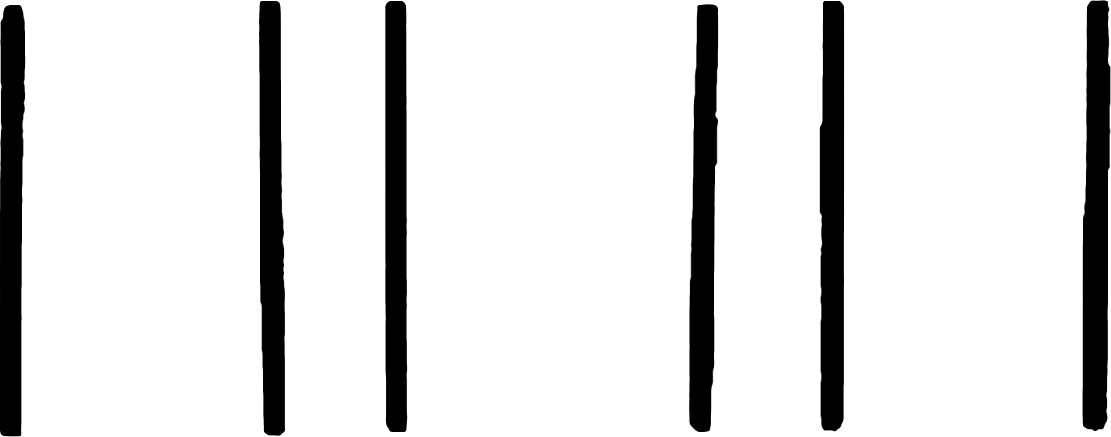
\includegraphics[width=3in]{img/strokes}\vskip 0.7em\par}} \\
are there two groups of three, or four sets of singles and pairs?\footnote{Or, much worse, are there three bracketed gaps?})

And, how does this interact with the compulsion to recognize that a derivation is legal?

Referring once again to the canard that mathematics can be explained by analogy with chess, chess is defined by rules \textbf{which depend on naive arithmetic and logic for their expression.} Moreover, mathematics is obviously not chess because mathematics is infinitary.

Could chaos in ordainment make a preposterous move legal?---or would it just cancel the system? Suppose one considers the rules of chess meaningless; or considers the claim that chess rules are meaningful to be inconsistent. Are matters then so chaotic that Kt--K6 is arguably legal as an opening move?

(Regarding chess, judgments of legality are fluid, negotiable---as they are in mathematics. Rules are altered in connection with tournament play. Also, the possible wins in chess change when very long, unintuitive games are allowed.)

\jarule

Nicholas Goodman says that it may not be true that all natural numbers are either prime or not---because for very large specific numbers the determination is too long to actually be done. So \enquote{unknowable} has to be added as a third truth-value.

But:
\begin{enumerate}[label=\arabic*), itemsep=1ex]
\item Merely adding \enquote{unknowable} as a third truth-value does not explicate Brouwer's logic---so that fails as a motivation.
\item The classical mathematician may reasonably say that it is much more convenient to idealize mathematical reality, and avoid the nuisance of the third truth-value, by imagining that all questions which extrapolate feasible questions in a homogeneous way have definite answers \enquote{known to God.} (Is that just mathematical induction?) You invent the mathematical universe this way because it is convenient or elegant.
\end{enumerate}

Can it then be guaranteed that structures which are trans-feasible and chosen for elegance will preclude $\vdash A$ and $\vdash\lnot A$? \enquote{Assuming that every question (including \enquote{infeasible} ones) has exactly one answer will not produce an inconsistency.}

Brouwer sought to prove that if the conventional classical assumption is made that \enquote{questions we cannot answer have definite answers for God,} one can get counter-examples to mandatory tenets of classical analysis. Classical mathematicians hit back by rejecting the key step in Brouwer's proof as illegal.

Goodman's objection to Brouwer is that Brouwer has a capricious attitude which itself doesn't take care to exclude inconsistency. But the same complaint is made against classical mathematics and its attitude of \enquote{Why not posit that all mathematical questions already have answers every though we don't know the answers now and may never know them?}

\jarule

The only rationale of mathematics which foundations of mathematics is prepared to defend metaphysically is formalism. (I don't mean that most twentieth-century mathematicians are formalists; I mean that Platonists such as Frege himself were not prepared to be forthright prophets of the supra-terrestrial world. \enquote{Chain of being} doctrines were expounded only by theosophists.) More narrowly, foundations of mathematics is prepared to champion only a concept of whole numbers relative to which the notion of a number's magnitude is meaningless. (Again, that doesn't mean that mathematicians don't hold far more traditional beliefs.)

It was when I offered concept art to some mathematical logicians that I ran into the real loyalties, which are atavistically traditional and theological. (Particularly when I presented \essaytitle{1966 Mathematical Studies} to Peter Ungar at Courant Institute in 1967, also when I presented it to Dennis Johnson at the Institute for Advanced Study in 1970. One may also consult the writings on foundations of mathematics by my schoolmate Nicholas Goodman.)

When one composes truly uninterpreted calculi (calculi which do not point to a naive-arithmetical interpretation)---or when one defines whole numbers which have the \enquote{wrong} magnitudes---then professional mathematicians want no part of the exercise.

\section{Bibliography}
\begin{hangparas}{2em}{1}

 Aristotle, \booktitle{Metaphysics}

 Michael Beeson, \booktitle{Foundations of Constructive Mathematics} (1985)

 Eric T. Bell, \booktitle{The Development of Mathematics} (1945)

 P. Benacerraf \& H. Putnam, eds., \booktitle{Philosophy of Mathematics} (1964)

 P. Bernays, \booktitle{Sur le platonisme} (1935)

 E.W. Beth, \papertitle{Remarks on Intuitionistic Logic,} in A. Heyting, ed., \booktitle{Constructivity in Mathematics} (1959)

 Errett Bishop \papertitle{Mathematics as a Numerical Language} in \booktitle{Intuitionism and Proof Theory}, ed. A. Kino, J. Myhill, \& R.E. Vesley (1970)

 David Bloor, \booktitle{Knowledge and Social Imagery} (1976)

 Bernard Bolzano, \booktitle{Paradoxes of the Infinite} (tr. 1950)

 L.E.J. Brouwer, \papertitle{The Rejected Parts of Brouwer's Dissertation on the Foundations of Mathematics,} \booktitle{Historica Mathematica 6} (1979)

 L.E.J. Brouwer, \booktitle{Collected Works, Vol. 1}

 George Spencer Brown, \booktitle{Laws of Form} (1979)

 Rudolf Carnap, \papertitle{The Elimination of Metaphysics Through Logical Analysis of Language,} in \booktitle{Logical Positivism}, ed. A.J. Ayer (1959)

 Rudolf Carnap, \papertitle{Pseudoproblems in Philosophy,} in \booktitle{The Logical Structure of the World} (tr. 1967)

 Rudolf Carnap, \booktitle{Logical Syntax of Language} (1937)

 Rudolf Carnap, \booktitle{Meaning and Necessity} (2nd ed., 1956)

 Felix Cleve, \booktitle{The Giants of Pre-Sophistic Greek Philosophy} (1965) B188.C55

 Richard Dedekind, \booktitle{Essays on the Theory of Numbers} (1901)

 J.J. de Iongh, \papertitle{Restricted Forms of Intuitionistic Mathematics,} in Evert Beth, ed., \booktitle{Proceedings of the Xth International Congress of Philosophy} (1949)

 Ren\'{e} Descartes, \papertitle{Rules for the Direction of the Mind,} in \booktitle{The Philosophical Writings of Descartes, Vol. I} (1985)

 Michael Dummett, \booktitle{Elements of Intuitionism} (1977), pp. 10--11

 Euclid, \booktitle{Elements} (tr. 1956, 2nd ed.)

 Paul Finsler, \papertitle{Gibt es unentscheidbare s\"{a}tze,} in \booktitle{Commentarii mathematici Helvetici} (1944), pp. 310--320, reviewed by Alonzo Church in \journaltitle{Journal of Symbolic Logic}, Vol. 11, pp. 131--132

 Gottlob Frege, \booktitle{The Foundations of Arithmetic} (tr. 1950)

 Gottlob Frege, selections from \booktitle{Grundgesetze der Arithmetik}, in \booktitle{Translations from the Philosophical Writings of Gottlob Frege} (2nd ed., 1960)

 Hans Freudenthal, \booktitle{Lincos: Design of a Language for Cosmic Intercourse} (1960)

 James Gleick, \papertitle{Machine Beats Man On Ancient Front}, \journaltitle{The New York Times}, August 26, 1986, p. C1 (about Dr. Kenneth Thompson, AT\&T Bell Laboratories, Murray Hill, New Jersey)

 Nicolas Goodman, \papertitle{Mathematics as an Objective Science}, \journaltitle{American Mathematical Monthly} (1979), pp. 540--551

 Nicolas Goodman in F. Richman, \booktitle{ed., Constructive Mathematics} (1981)

 R.L. Goodstein, \booktitle{Constructive Formalism} (1951)

 I . Grattan-Guinness, \booktitle{The Development of the Foundations of Mathematical Analysis from Euler to Riemann} (MIT, 1970)

 Emil Grosswald, \booktitle{Topics from the Theory of Numbers} (1966), pp. 27--8

 Thomas Heath, \booktitle{A History of Greek Mathematics} (1921)

 Thomas Heath, \booktitle{Mathematics in Aristotle} (1949)

 Arend Heyting, \booktitle{Intuitionism: An Introduction} (1971)

 David Hilbert, \booktitle{Foundations of Geometry}

 David Hilbert \& P. Bernays, \booktitle{Grundlagen der Mathematik} (1934-39)

 David Hilbert \& W. Ackermann, \booktitle{Principles of Mathematical Logic} (1950)

 Edmund Husserl, \booktitle{Philosophie der Arithmetik} (1891)

 Edmund Husserl, \journaltitle{G\"{o}ttinger gelehrte Anzeigen}, 1891, No. 7, p. 272 \linebreak{}
 [Husserl attacks the empty set]

 Edmund Husserl, \booktitle{The Phenomenology of Internal Time-Consciousness}, tr. James Churchill (Bloomington, 1964)

 Morris Kline, \booktitle{Mathematical Thought from Ancient to Modern Times} (1972)

 G.T. Kneebone, \booktitle{Mathematical Logic and the Foundations of Mathematics} (1963)

 Imre Lakatos, ed., \booktitle{Problems in the Philosophy of Mathematics} (1967)

 Imre Lakatos, \booktitle{Mathematics, Science, and Epistemology} (1978)

 \booktitle{Logic, Methodology, and Philosophy of Science}, ed. Nagel, Suppes, and Tarski (1962)

 Andrei A. Markov, \booktitle{Theory of Algorithms} (1961)

 Gregory Moore, \booktitle{Zermelo's Axiom of Choice} (1982)

 Jan Mycielski, \papertitle{Analysis Without Actual Infinity}, \journaltitle{Journal of Symbolic Logic}, Vol. 46, p. 625

 Edward Nelson, \booktitle{Predicative Arithmetic} (1986)

 Plato, \booktitle{Meno}

 Plato, \booktitle{Philebus}

 Plato, \booktitle{Timeaus}

 Emil Post in Martin Davis, ed., \booktitle{The Undecidable} (1964)

 Proclus, \booktitle{A Commentary on the First Book of Euclid's Elements}, tr. Glenn Morrow (1970)

 W.V.O. Quine, \booktitle{Mathematical Logic} (revised)

 W.V.O. Quine, \booktitle{Methods of Logic}

 Frank P. Ramsey, \booktitle{The Foundations of Mathematics} (1931)

 Hans Reichenbach, \booktitle{Elements of Symbolic Logic} (1947)

 Michael Resnik, \booktitle{Frege and the Philosophy of Mathematics} (1980)

 Gabriel Stolzenberg, \papertitle{Can an Inquiry into the Foundations of Mathematics Tell Us Anything Interesting about Mind?}, in \journaltitle{Psychology and Biology of Language and Thought} (1978)

 Alfred Tarski, \booktitle{Logic, Semantics, Metamathematics} (1956)

 Alfred Tarski, \papertitle{The Semantic Conception of Truth,} \journaltitle{Philosophy and Phenomenological Research 4} (1944)

 Dirk van Dalen, \booktitle{Logic and Structure} (1983)

 D. van Dantzig, \papertitle{Comments on Brouwer's Theorem on Essentially-negative Predicates}, \journaltitle{Indagationes Mathematicae}, Vol. 11, pp. 347--55

 Jean van Heijenoort, ed., \booktitle{From Frege To Godel} (1967)

 B. van Rootselaar, \papertitle{On Subjective Mathematical Assertions}, \booktitle{Intuitionism and Proof Theory}, ed. A. Kino, J. Myhill, \& R.E. Vesley (1970)

 C.F. von Weizsäcker, \booktitle{The Unity of Nature} (1980), pp. 78-9

 Stan Wagon, \booktitle{The Banach-Tarski Paradox} (1985)

 Hermann Weyl, \booktitle{Philosophy of Mathematics and Natural Science} (1949)

 Leslie A. White, \papertitle{The Locus of Mathematical Reality: An Anthropological Footnote,} in J.R. Newman, ed., \journaltitle{The World of Mathematics}, Vol. 4

 A. Whitehead and B. Russell, \booktitle{Principia Mathematica}

 Ludwig Wittgenstein, \booktitle{Wittgenstein's Lectures on the Foundations of Mathematics} (1976)

 Ludwig Wittgenstein, \booktitle{Philosophical Grammar} (1974)

Ludwig Wittgenstein, \booktitle{Remarks on the Foundations of Mathematics} (1978 ed.)
\end{hangparas}


